\question{Молекулярные спектры. Комбинационное рассеяние света.}

\subquestion{Молекулярные спектры}
В отличии от атомных спектров состоящих из отдельных линий, молекулярные 
спектры состоят из отдельных полос, каждый из которых состоит из большого 
числа тесно расположенных линий (отсюда пошло название полосатые спектры). 
Различают три вида полос, в зависимости от энергии обуславливающей их:
\begin{enumerate}
    \item электронно-колебательные полосы
    \item вращательные полосы
    \item колебательно-вращательные полосы
\end{enumerate}

При электронном переходе \( E'_e \rightarrow E''_e \) изменяется 
электронная конфигурация оболочки, следовательно изменяется сила 
действующая между ядрами, следовательно меняется и колебательная и 
вращательная энергии. То есть при электронном переходе меняются все три 
составляющие энергии и вместо одной линии соответствующую переходу 
\( E'_e \rightarrow E''_E \) появляется целая полоса частот. Как 
показывает измерение электронные переходы совершаются за время 
\( t \sim 10^{-15} \) сек., а характерные периоды колебаний ядер молекулы 
имеют \( \sim 10^{-10}, 10^{-15} \). Этот факт является основой принципа 
Франка-Кондона: \emph{электронный переход происходит наиболее вероятно без 
изменения положений ядер молекулы.} 

\begin{figure}[h!]
    \center
    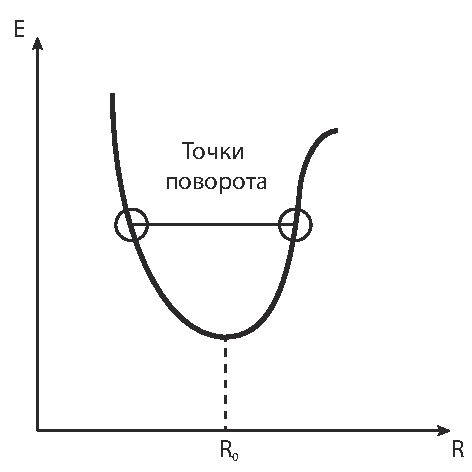
\includegraphics[width=.47\textwidth]{16_01}
\end{figure}

Вероятность нахождения атома в данной точке пространства пропорционален 
времени нахождения в окрестности этой точки и соответственно обратно 
пропорционален скорости движения. В окрестности точки поворота, скорости 
значительно меньше, чем в центре, поэтому больше времени атомы в молекулах 
проводят в конфигурации, когда полная энергия практически равна 
потенциальной, а кинетическая примерно равна нулю. Поэтому вероятность 
испускания или поглощения фотона наибольшее тогда, когда ядры неподвижны 
или движутся медленно.

Рассмотрим два электронных перехода: 
\begin{figure}[h!]
    \center
    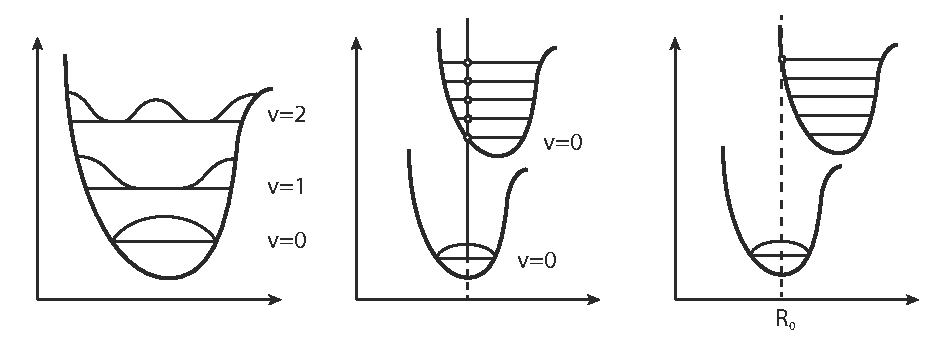
\includegraphics[width=.47\textwidth]{16_02}
\end{figure}

При электронных переходах:
\begin{enumerate}
    \item изменяется электронная конфигурация атома, 
    входящего в молекулу; 
    \item изменяются всех три составляющих энергии молекулы; 
    \item спектр очень <<сложный>>;
    \item наибольшей интенсивностью обладают линии подчиняющиеся принципу 
    Франка-Кондана;
\end{enumerate}

Вращательная полоса возникает при переходах между вращательными уровнями 
(при этом электронная конфигурация и энергия колебаний не изменяется)
\[ 
    \hbar\omega = \Delta E_r = \frac{\hbar^2}{2I} J'(J'+1) - 
    \frac{\hbar^2}{2I} J(J+1)
\]
\[ J' = J + 1 \text{ (в случае испускании фотона)} \]
\[ 
    \omega = \frac{\hbar}{2I}(J+1)(J+2) - \frac{\hbar}{2I}J(J+1) = 
    \frac{\hbar}{I}(J+1)
\]
\[ 
    J = 0, 1, 2, ...
\]
Частоты соответствующие этим квантовым числам соответственно:
\[ 
    \omega_1 = \frac{\hbar}{I}; \quad
    \omega_2 = \frac{2\hbar}{I} = 2\omega_1; \quad
    \omega_3 = \frac{3\hbar}{I} = 3\omega_1; ...
\]

Вращательный спектр состоит из ряда равноотстоящих линий расположенных в 
далёкой инфракрасной области. Измеряя расстояние между линиями мы можем 
определить момент инерции молекулы.

Колебательно-вращательные полосы возникают при изменении колебательной и 
вращательной энергии молекулы (в пределах данной электронной конфигурации 
существует правило отбора \( \Delta v = \pm 1 \).
\[ 
    \hbar\omega = \Delta E_v + \Delta E_R = 
    \left(v' + \frac{1}{2}\right)\omega_v\hbar - 
    \left(v + \frac{1}{2}\right)\omega_v\hbar + 
    \frac{\hbar^2}{2I}J'(J'+1) - \frac{\hbar^2}{2I}J(J+1)
\]

Рассмотрим процесс излучения фотона:
\[ 
    v' = v + 1; \quad
    J' = J \pm 1
\]
\begin{enumerate}
    \item \( J' = J + 1 \)
        \[ \omega = \omega_v + \frac{\hbar}{I}(J+1) \]
        \[ 
            J = 0, 1, 2, ...; \quad
            \Delta\omega_r = \omega_1, \omega_2, \omega_3, ...
        \]
    \item \( J' = J - 1 \)
        \[ 
            \Delta\omega_r = \frac{\hbar}{2I}
            \left(J(J-1) - J(J+1)\right) = -\frac{\hbar}{I}J
        \]
        \[ J = 1, 2, ... \]
        \[ \Delta\omega_r = -\omega, -2\omega, -3\omega \]
        \[ \omega = \omega_v \pm \frac{\hbar}{I}k,\quad k = 1, 2, 3 ... \]
\end{enumerate}

\begin{figure}[h!]
    \center
    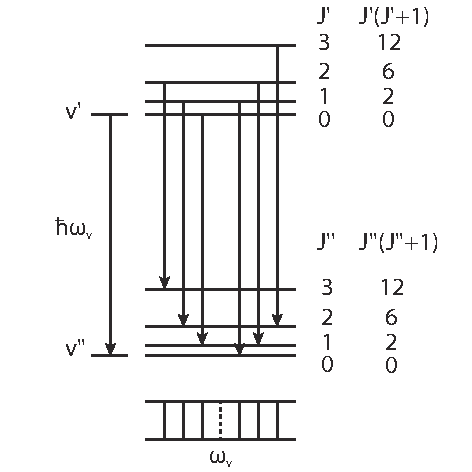
\includegraphics[width=.47\textwidth]{16_03}
\end{figure}

Колебательная вращательная полоса состоит из совокупности симметричных 
относительно \( \omega_v \) линий отстоящих друг от друга на расстояние 
\( \Delta\omega = \omega_1 = \hbar/I \).

Заметим, что вращательная и колебательно-вращательная полосы наблюдаются 
на опыте, только для не симметричных молекул, то есть для молекул из 
различных атомов. У симметричных молекулы дипольный момент равна нулю, 
что приводит к запретам колебательных и вращательных переходов.

\subquestion{Комбинационное рассеяние света}
Комбинационное рассеяние света или КРС -- это явление заключается в том, 
что в спектре рассеяние возникают при прохождении света через газы, 
жидкости или прозрачные кристаллические тела, помимо первоначальной линии 
появляются новые линии, частоты которых представляют собой комбинации 
частоты падающего света \( \omega_0 \) и частоты \( \omega_i \) 
колебательной или вращательной частот рассеивающих молекул.
\[ \omega = \omega_0 \pm \omega_i \]
\[ 
    \omega = \omega_0 - \omega_i, \lambda = \lambda_0 + \lambda_i 
    \text{ -- красные спутники}
\]
\[ 
    \omega = \omega_0 + \omega_i, \lambda = \lambda_0 - \lambda_i
    \text{ -- фиолетовые спутники}
\]

\emph{Природа возникновения: } это процесс неупругого столкновения фотонов 
с молекулами, при соударении фотон может отдать молекуле или получить от 
неё, только такое количество энергии, которые равны разностям двух 
энергетическим уровням. Если при столкновении энергия молекулы 
увеличивается на \( \Delta E = E'' - E' \), то энергия фотона станет 
равной \( E_0 - \Delta E \) соответственно частота фотона уменьшится на 
величину \( \Delta E / \hbar \) -- возникает красный спутник. Если же 
молекула находилась в возбужденном состоянии с энергией \( E'' \), то 
она в результате столкновения может перейти в \( E' \) и отдать избыток 
энергии фотону -- фиолетовый спутник.

Рассеяние фотона сопровождается переходами молекулы между различными 
колебательными и вращательными уровнями в результате возникает ряд 
симметрично расположенных спутников. 

При обычных температурах согласно распределению Больцмана, число молекул 
в возбужденных состояниях значительно меньше, чем в основном поэтому в 
основном будут происходить процессы поглощения энергии и значит 
интенсивность красных спутников будет выше. При высоких температурах 
они сравняются.

Спектры КРС настолько характерны для молекул, что с их помощью осуществляют 
анализ сложных молекулярных смесей, анализ химическими методами 
которых сильно затруднён или невозможен.

\newpage
